\UC{Aggiunta nuovo prodotto}
% \begin{figure}[H]
%     \centering
%     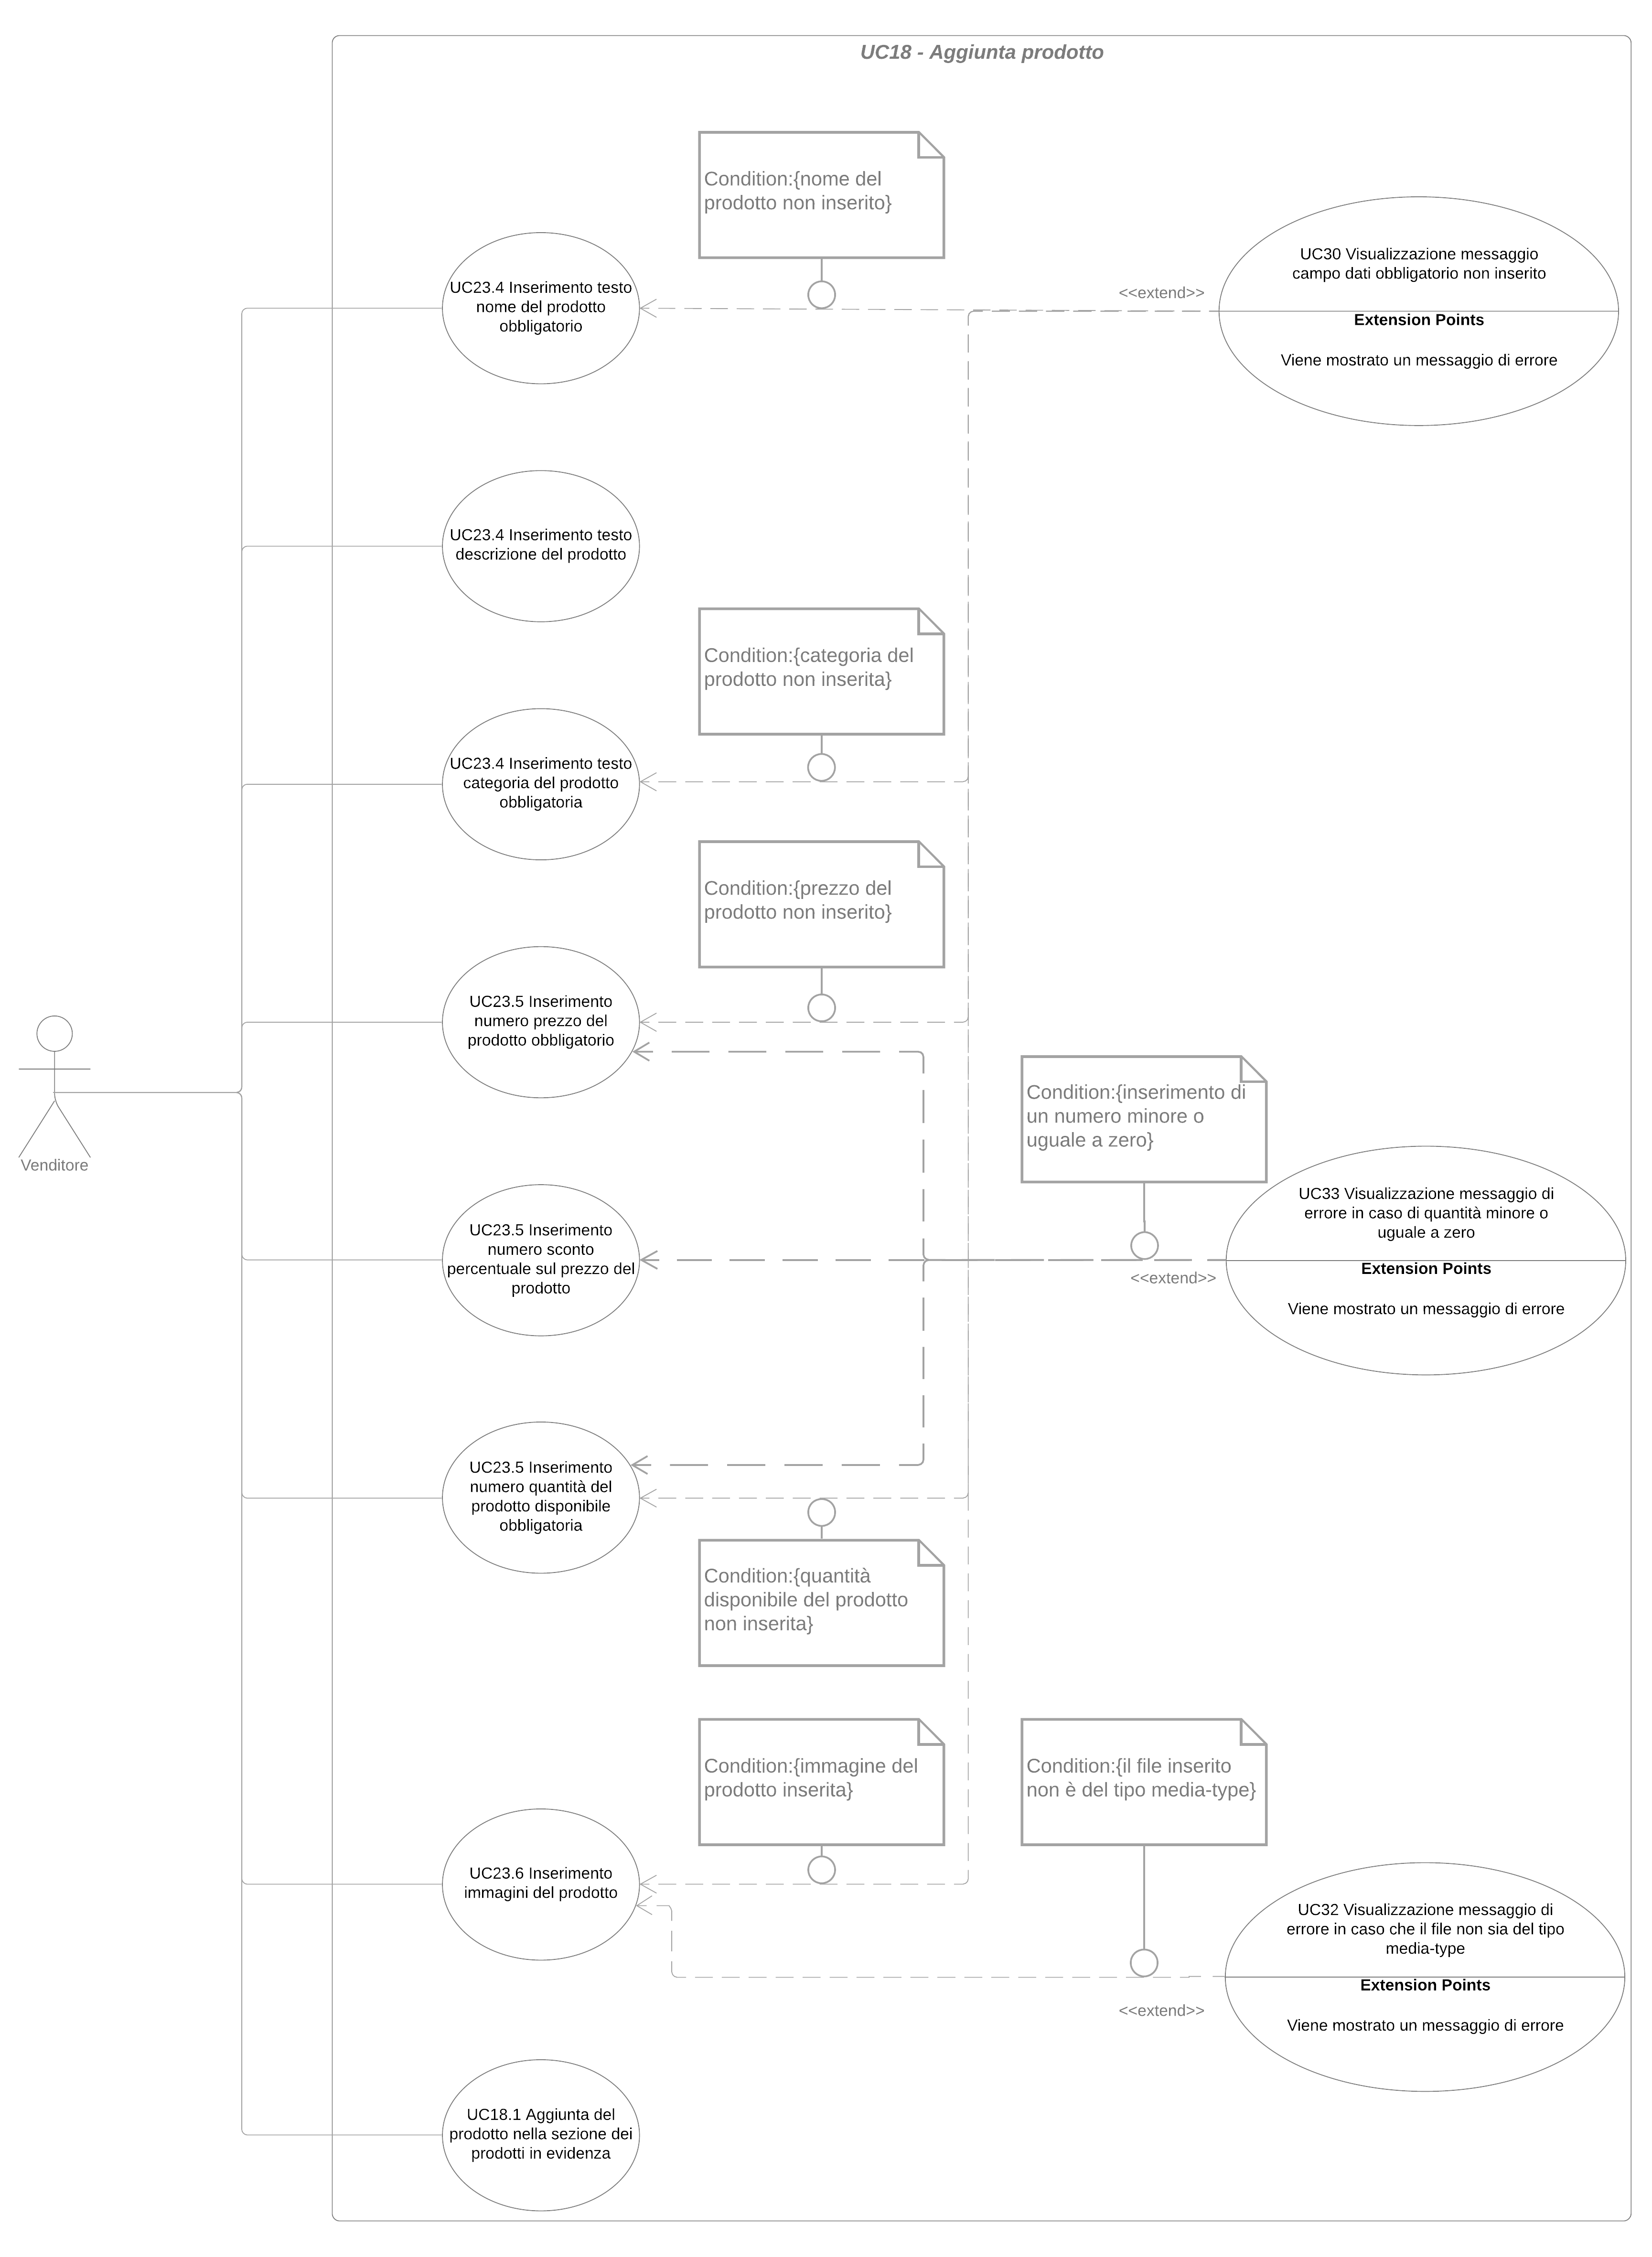
\includegraphics[scale=0.1]{Immagini/DiagrammiUC/UC18AggiuntaProdotto.png}
%     \caption{Diagramma di \actualUC: Aggiunta di un prodotto nella piattaforma da parte del venditore} 
%     \label{fig:AggiuntaProdotto}
% \end{figure}

Il venditore aggiunge un nuovo prodotto alla piattaforma, così da poter essere venduto.
\begin{itemize}
    \item \textbf{Attori primari:} venditore;
    \item \textbf{Precondizione:} il venditore si trova nella vista della \glo{dashboard} e seleziona l'azione di aggiunta di un prodotto;
    \item \textbf{Postcondizione:} il venditore ha aggiunto il prodotto nella piattaforma;
    \item \textbf{Scenario principale:} Il venditore preme sull'azione che porta alla vista di aggiunta di un prodotto e compie le seguenti azioni:
    \begin{itemize}
        \item (\actualUC.1) - Inserimento del nome del prodotto;
        \item (\actualUC.2) - Inserimento della descrizione del prodotto;
        \item (\actualUC.3) - Inserimento delle categorie del prodotto;
        \item (\actualUC.4) - Inserimento del prezzo del prodotto;
        \item (\actualUC.5) - Inserimento dello sconto percentuale al prezzo del prodotto;
        \item (\actualUC.6) - Inserimento della quantità del prodotto disponibile in magazzino;
        \item (\actualUC.7) - Inserimento delle foto del prodotto;
        \item (\actualUC.8) - Scelta di aggiunta del prodotto tra quelli in evidenza;
        \item Conferma gli inserimenti e aggiunge il prodotto alla piattaforma.
    \end{itemize}
\end{itemize}

\resetSubUC
\subUC{Inserimento del nome del prodotto}
Il venditore inserisce il nome del prodotto da aggiungere.
\begin{itemize}
    \item \textbf{Attori primari:} venditore;
    \item \textbf{Precondizione:} il venditore si trova nella vista di aggiunta di un nuovo prodotto;
    \item \textbf{Postcondizione:} il venditore ha inserito il nome del prodotto;
    \item \textbf{Scenario principale:} il venditore si trova nella vista di aggiunta di un nuovo prodotto ed inserisce il nome del prodotto.
    \item \textbf{Estensioni:} 
    \begin{enumerate}
    	\item Il venditore non inserisce il nome del prodotto. In questo caso:
	    \begin{itemize}
	        \item (UC) - Verrà visualizzato il messaggio di errore campo dati obbligatorio non inserito.
	        \item Verrà impedita l'aggiunta del nuovo prodotto.
	    \end{itemize}
	\end{enumerate}
\end{itemize}

\subUC{Inserimento della descrizione del prodotto}
Il venditore inserisce la descrizione del prodotto da aggiungere.
\begin{itemize}
    \item \textbf{Attori primari:} venditore;
    \item \textbf{Precondizione:} il venditore si trova nella vista di aggiunta di un nuovo prodotto;
    \item \textbf{Postcondizione:} il venditore ha inserito la descrizione del prodotto;
    \item \textbf{Scenario principale:} il venditore si trova nella vista di aggiunta di un nuovo prodotto ed inserisce la descrizione del prodotto;
    \item \textbf{Estensioni:}
    \begin{enumerate}
    	\item Il venditore non inserisce la descrizione del prodotto. In questo caso:
    	\begin{itemize}
    		\item (UC) - Verrà visualizzato il messaggio di errore campo dati obbligatorio non inserito;
    		\item Verrà impedita la conferma di aggiunta del prodotto.
    	\end{itemize}
    \end{enumerate}
\end{itemize}

\subUC{Inserimento delle categorie del prodotto}
Il venditore inserisce le categorie del prodotto da aggiungere.
\begin{itemize}
    \item \textbf{Attori Primari:} venditore;
    \item \textbf{Precondizione:} il venditore si trova nella vista di aggiunta di un nuovo prodotto;
    \item \textbf{Postcondizione:} il venditore ha inserito le categorie del prodotto;
    \item \textbf{Scenario principale:} il venditore si trova nella vista di aggiunta di un nuovo prodotto ed inserisce le categorie a cui fa parte il prodotto, prendendole dalla lista di categorie disponibili;
    \item \textbf{Estensioni:}
    \begin{enumerate}
    	\item Il venditore non ha inserito alcuna categoria e il prodotto viene automaticamente categorizzato come senza categoria.
    \end{enumerate}
\end{itemize}

\subUC{Inserimento del prezzo del prodotto}
Il venditore inserisce il prezzo a cui vendere il prodotto da aggiungere.
\begin{itemize}
    \item \textbf{Attori primari:} venditore;
    \item \textbf{Precondizione:} il venditore si trova nella vista di aggiunta di un nuovo prodotto;
    \item \textbf{Postcondizione:} il venditore ha inserito il prezzo a cui vendere il prodotto;
    \item \textbf{Scenario principale:} il venditore si trova nella vista di aggiunta di un nuovo prodotto ed inserisce il prezzo a cui vendere il prodotto;
    \item \textbf{Estensioni:}
    \begin{enumerate}
    	\item Il venditore non inserisce il prezzo del prodotto. In questo caso:
    	\begin{itemize}
    		\item (UC) - Verrà visualizzato il messaggio di errore campo dati obbligatorio non inserito;
    		\item Verrà impedita l'aggiunta del nuovo prodotto.
    	\end{itemize}
    	\item Il venditore inserisce un prezzo minore o uguale a zero. In questo caso:
    	\begin{itemize}
    		\item (UC) - Verrà visualizzato il messaggio di errore prezzo minore o uguale a zero;
    		\item Verrà impedita l'aggiunta del nuovo prodotto.
    	\end{itemize}
    \end{enumerate}
\end{itemize}

\subUC{Inserimento dello sconto percentuale al prezzo del prodotto}
Il venditore inserisce lo sconto percentuale da applicare al prezzo del prodotto da aggiungere.
\begin{itemize}
    \item \textbf{Attori primari:} venditore;
    \item \textbf{Precondizione:} il venditore si trova nella vista di aggiunta di un nuovo prodotto;
    \item \textbf{Postcondizione:} il venditore ha inserito lo sconto percentuale da applicare al prezzo del prodotto;
    \item \textbf{Scenario principale:} il venditore si trova nella vista di aggiunta di un nuovo prodotto ed inserisce lo sconto percentuale da applicare al prezzo del prodotto. In seguito il prezzo a cui vendere quel prodotto sarà scontato della percentuale applicata;
    \item \textbf{Estensioni:}
    \begin{enumerate}
    	\item Nel caso in cui il venditore non inserisca alcunché, allora non verrà applicato alcuno sconto;
    	\item Il venditore inserisce uno sconto maggiore di 100\%. In questo caso:
    	\begin{itemize}
    		\item (UC) - Verrà visualizzato il messaggio di errore in caso di sconto maggiore di 100\%;
    		\item Verrà impedita l'aggiunta del nuovo prodotto.
    	\end{itemize}
    	\item Il venditore inserisce uno sconto minore di zero. In questo caso:
    	\begin{itemize}
    		\item (UC) - Verrà mostrato un messaggio di errore con la segnalazione della causa;
    		\item Verrà impedita l'aggiunta del nuovo prodotto.
    	\end{itemize}
    \end{enumerate}
\end{itemize}

\subUC{Inserimento della quantità del prodotto disponibile in magazzino}
Il venditore inserisce la quantità disponibile attualmente in magazzino del prodotto da aggiungere.
\begin{itemize}
    \item \textbf{Attori primari:} venditore;
    \item \textbf{Precondizione:} il venditore si trova nella vista di aggiunta di un nuovo prodotto;
    \item \textbf{Postcondizione:} il venditore ha inserito la quantità disponibile attualmente in magazzino del prodotto;
    \item \textbf{Scenario principale:} il venditore si trova nella vista di aggiunta di un nuovo prodotto ed inserisce la quantità disponibile attualmente in magazzino del prodotto;
    \item \textbf{Estensioni:}
    \begin{enumerate}
    	\item Nel caso in cui il venditore inserisca 0 come disponibilità attuale, allora il prodotto verrà indicato come non disponibile.
    	\item Il venditore inserisce una quantità minore o uguale a zero. In questo caso:
    	\begin{itemize}
    		\item (UC) - Verrà visualizzato il messaggio di errore quantità minore o uguale a zero;
    		\item Verrà impedita l'aggiunta del nuovo prodotto.
    	\end{itemize}
    	\item Il venditore non inserisce la quantità del prodotto. In questo caso:
    	\begin{itemize}
    		\item (UC) - Verrà visualizzato il messaggio di errore campo dati obbligatorio non inserito;
    		\item Verrà impedita l'aggiunta del nuovo prodotto.
    	\end{itemize}
    \end{enumerate}
\end{itemize}

\subUC{Inserimento foto del prodotto}
Il venditore inserisce le foto relative al prodotto da aggiungere.
\begin{itemize}
    \item \textbf{Attori primari:} venditore;
    \item \textbf{Precondizione:} il venditore si trova nella vista di aggiunta di un nuovo prodotto;
    \item \textbf{Postcondizione:} il venditore ha inserito le foto relative al prodotto;
    \item \textbf{Scenario principale:} il venditore si trova nella vista di aggiunta di un nuovo prodotto ed inserisce massimo quattro foto relative al prodotto;
    \item \textbf{Estensioni:}
    \begin{enumerate}
    	\item Il venditore non inserisce alcuna foto del prodotto. In questo caso:
    	\begin{itemize}
    		\item (UC) - Verrà visualizzato il messaggio di errore nessuna foto inserita.
    		\item Verrà impedita l'aggiunta del nuovo prodotto.
    	\end{itemize}
    	\item Il venditore seleziona un file che non è del tipo immagine. In questo caso:
    	\begin{itemize}
    		\item (UC) - Verrà visualizzato il messaggio di errore il quale segnala che il file selezionato non è del tipo immagine.
    		\item Verrà impedita l'aggiunta del nuovo prodotto.
    	\end{itemize}
    	\item Il venditore cerca di inserire più di quattro foto relative ad un prodotto. In questo caso:
    	\begin{itemize}
    		\item (UC) - Verrà visualizzato il messaggio di errore il quale segnala il tentativo di aggiunta di più quattro foto relativa ad un prodotto.
    		\item Verrà impedita l'aggiunta del nuovo prodotto.
    	\end{itemize}
    \end{enumerate}
\end{itemize}

\subUC{Scelta di aggiunta del prodotto tra quelli in evidenza}
Il venditore decide se il prodotto è da inserire tra quelli in evidenza da visualizzare nella home.
\begin{itemize}
	\item \textbf{Attori primari:} venditore;
    \item \textbf{Precondizione:} il venditore si trova nella vista di aggiunta di un nuovo prodotto;
    \item \textbf{Postcondizione:} il venditore ha deciso se il prodotto è da inserire tra quelli in evidenza oppure no ed agisce di conseguenza;
    \item \textbf{Scenario principale:} il venditore si trova nella vista di aggiunta di un nuovo prodotto e lo aggiunge tra quelli in evidenza da visualizzare nella home;
    \item \textbf{Estensioni:}
    \begin{enumerate}
    	\item Il venditore decide di non inserire il prodotto tra quelli in evidenza e, per questo motivo, non compie alcuna azione.
    \end{enumerate}
\end{itemize}

%%%%%%%%%%%%%%%%%%%%%%%%%%%%%%%%%%%%%%%%%%%%%%%%%%%%%%%%%%%%%%%%%%%%%%%%%%%%%%%%%%%%%%%%%%%%%%%%%%%%%%%%%%%%%%%%%%%%%%%%%%%%%%%%%%%%%%%%%%%%%%%%%%%%%%%%%%%%%%%%%%%%%%%%%%%%%%%%%%%%%%%%%%%%%%

\UC{Modifica informazioni del prodotto}
% \begin{figure}[H]
%     \centering
%     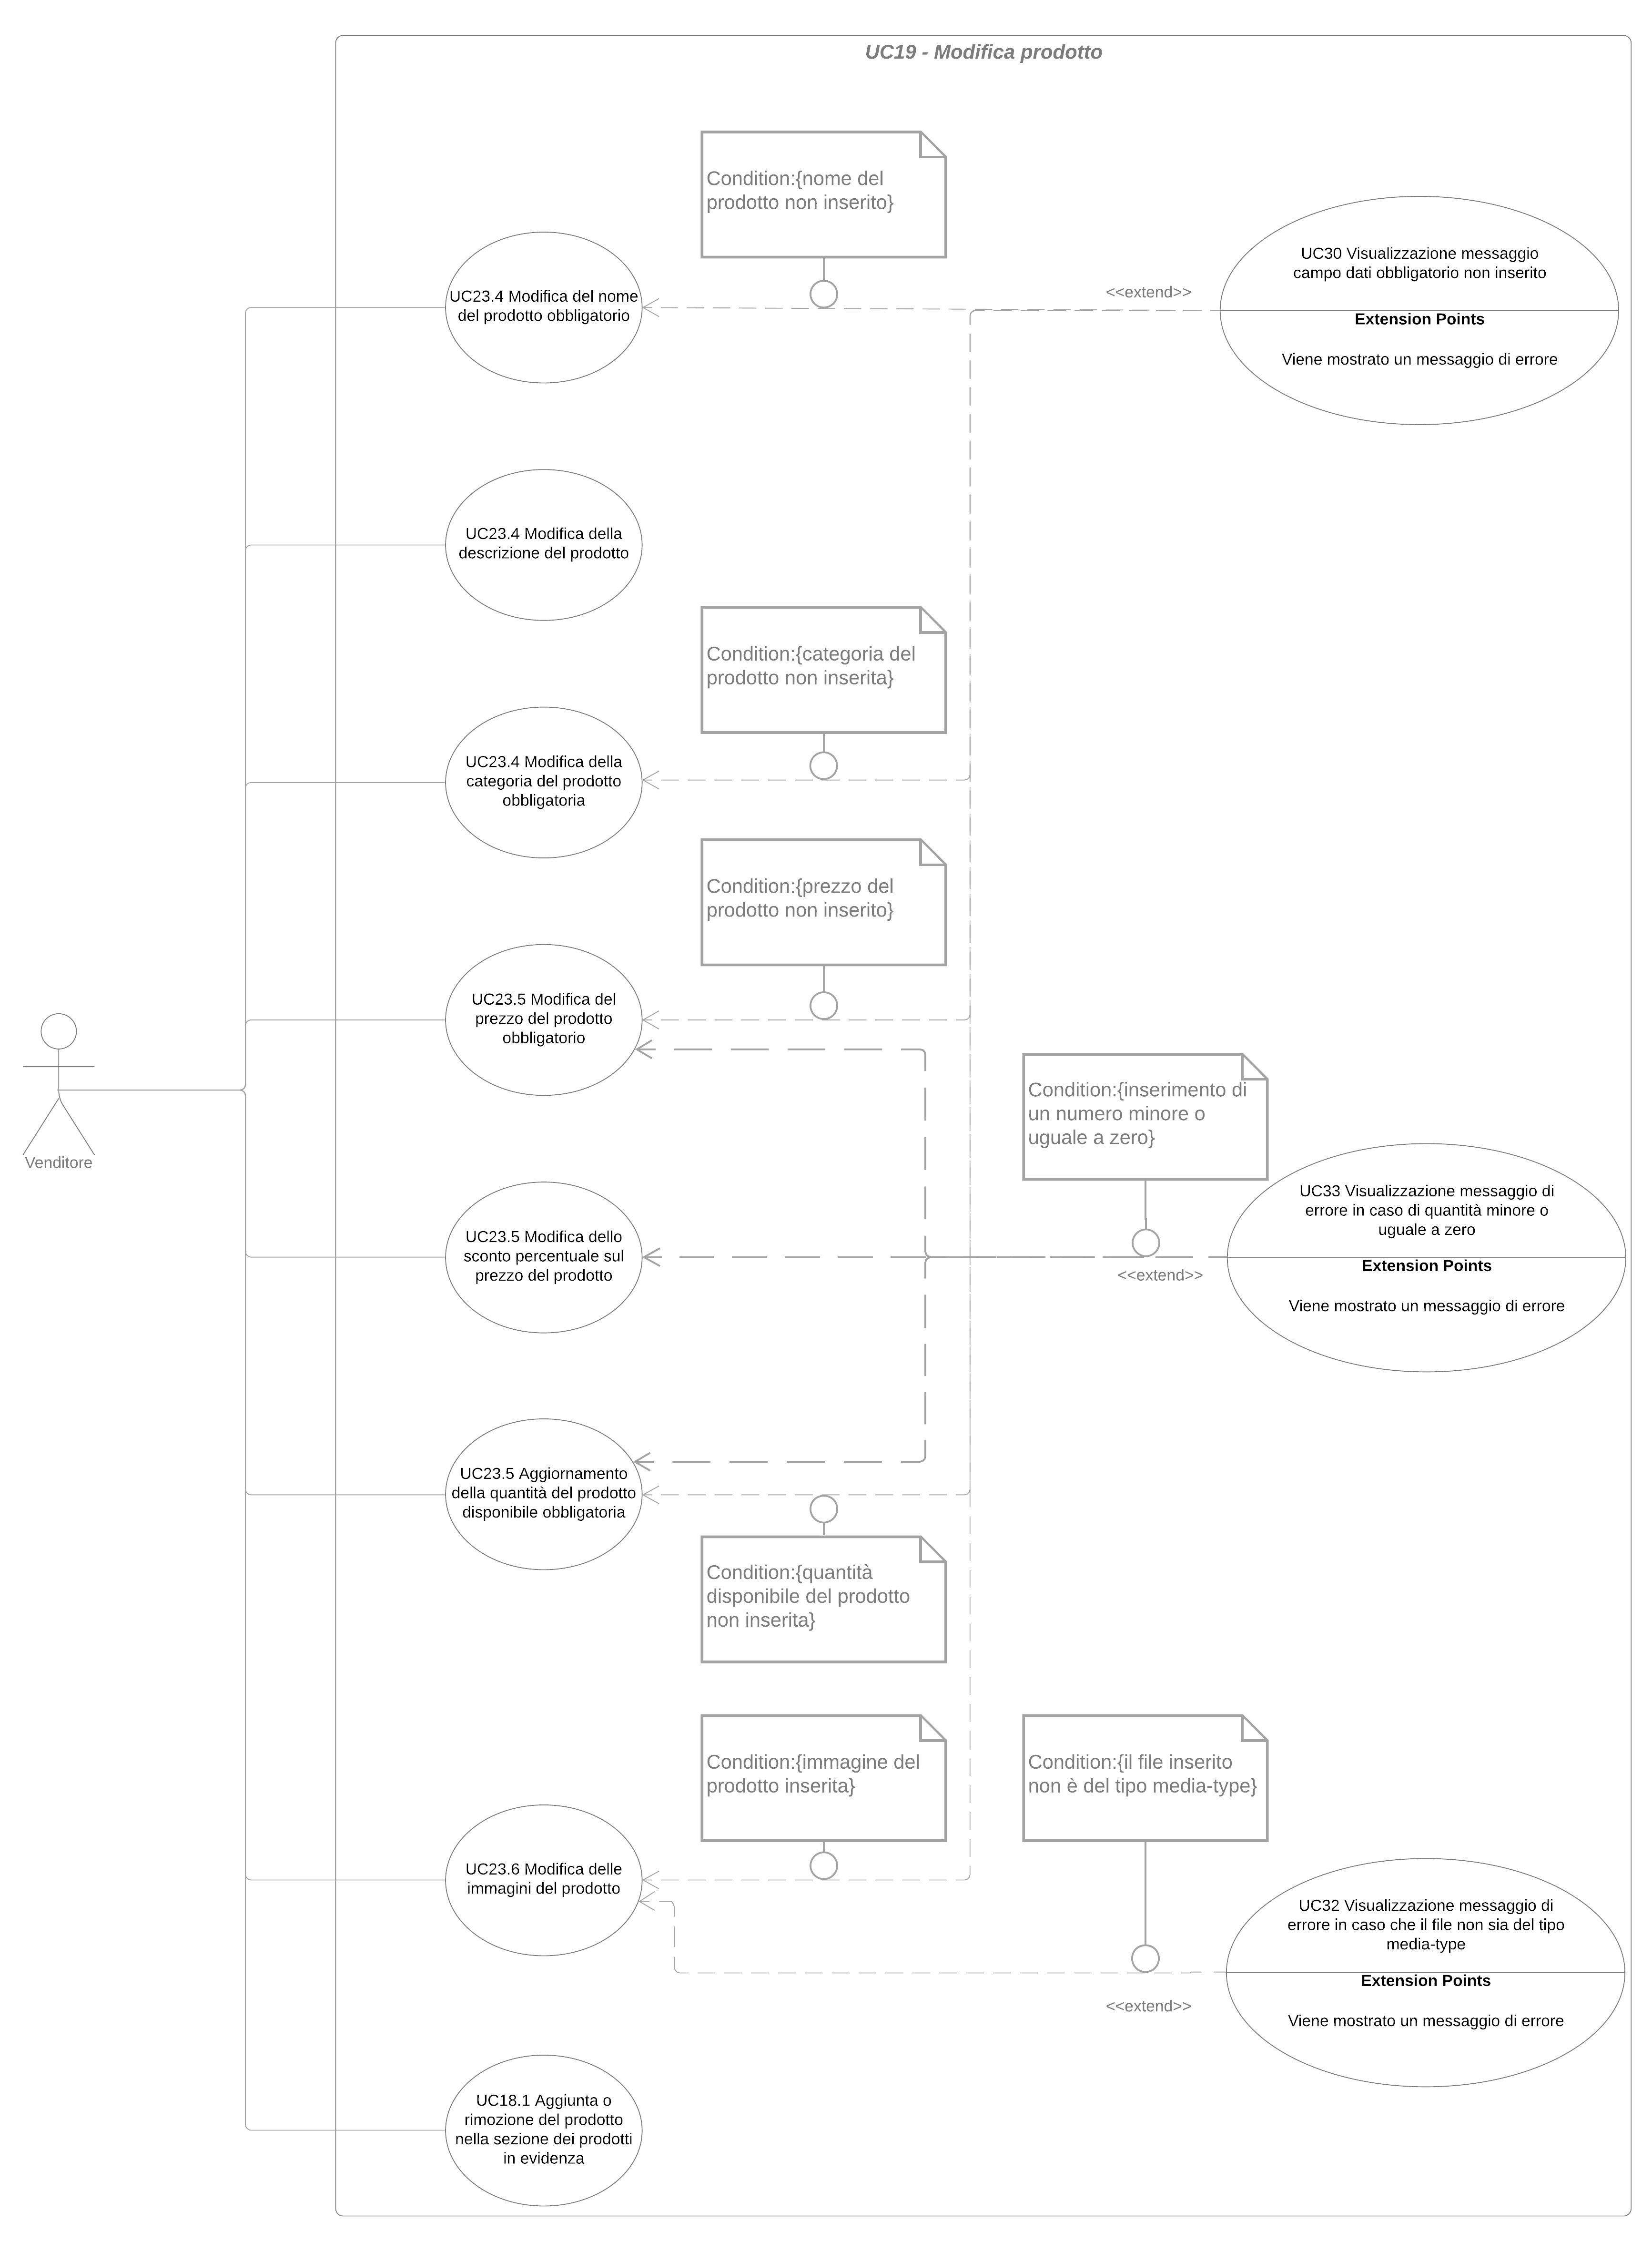
\includegraphics[scale=0.1]{Immagini/DiagrammiUC/UC19ModificaProdotto.png}
%     \caption{Diagramma di \actualUC: Modifica di un prodotto nella piattaforma da parte del venditore}
%     \label{fig:ModificaProdotto}
% \end{figure}

Il venditore modifica uno o più campi di un prodotto che è stato inserito nella piattaforma.
\begin{itemize}
    \item \textbf{Attori primari:} venditore;
    \item \textbf{Precondizione:} il venditore si trova nella PDP di un prodotto e seleziona l'azione di modifica di quel prodotto.
    \item \textbf{Postcondizione:} il venditore ha modificato il prodotto con le modifiche compiute.
    \item \textbf{Scenario principale:} il venditore seleziona l'azione che porta alla vista di modifica di un prodotto e compie zero, o più, delle seguenti azioni:
    \begin{itemize}
        \item (\actualUC.1) - Modifica del nome del prodotto;
        \item (\actualUC.2) - Modifica della descrizione del prodotto;
        \item (\actualUC.3) - Modifica delle categorie del prodotto;
        \item (\actualUC.4) - Modifica del prezzo del prodotto;
        \item (\actualUC.5) - Modifica dello sconto percentuale al prezzo del prodotto;
        \item (\actualUC.6) - Aggiunta di nuove foto del prodotto;
        \item (\actualUC.7) - Rimozione di foto del prodotto.
    \end{itemize}
    In seguito ci sarà la conferma delle modifiche compiute e il prodotto viene modificato;
    \item \textbf{Estensioni:}
    \begin{enumerate}
    	\item Il venditore non conferma le modifiche effettuate e perciò verranno scartate.
    \end{enumerate}
\end{itemize}

\resetSubUC
\subUC{Modifica del nome del prodotto}
Il venditore vuole modificare il nome del prodotto.
\begin{itemize}
    \item \textbf{Attori primari:} venditore;
    \item \textbf{Precondizione:} il venditore si trova nella vista di modifica del prodotto;
    \item \textbf{Postcondizione:} il venditore ha modificato il nome del prodotto;
    \item \textbf{Scenario Principale:} il venditore si trova nella vista di modifica del prodotto e modifica il nome attraverso i seguenti passi:
    \begin{itemize}
        \item Si posiziona nel campo di inserimento del nome del prodotto dove è presente quello attualmente utilizzato;
        \item Lo modifica.
    \end{itemize}
    \item \textbf{Estensioni:}
    \begin{enumerate}
    	\item Il venditore cancella il nome attuale del prodotto e lo lascia vuoto non scrivendone uno nuovo. In questo caso:
    	\begin{itemize}
    		\item (UC) - Verrà visualizzato il messaggio di errore campo dati obbligatorio non inserito.
    		\item Verrà impedita la conferma delle modifiche al prodotto.
    	\end{itemize}
    \end{enumerate}
\end{itemize}

\subUC{Modifica della descrizione del prodotto}
Il venditore vuole modificare la descrizione del prodotto.
\begin{itemize}
    \item \textbf{Attori primari:} venditore;
    \item \textbf{Precondizione:} il venditore si trova nella vista di modifica del prodotto;
    \item \textbf{Postcondizione:} il venditore ha modificato la descrizione del prodotto;
    \item \textbf{Scenario principale:} il venditore si trova nella vista di modifica del prodotto e modifica la descrizione attraverso i seguenti passi:
    \begin{itemize}
        \item Si posiziona nel campo di inserimento della descrizione del prodotto dove è presente quella attualmente utilizzata.
        \item La modifica.
    \end{itemize}
    \item \textbf{Estensioni:}
    \begin{enumerate}
    	\item Il venditore cancella la descrizione attuale del prodotto e la lascia vuota non scrivendone una nuova. In questo caso:
    	\begin{itemize}
    		\item (UC) - Verrà visualizzato il messaggio di errore campo dati obbligatorio non inserito.
    		\item Verrà impedita la conferma delle modifiche al prodotto.
    	\end{itemize}
    \end{enumerate}
\end{itemize}

\subUC{Modifica delle categorie del prodotto}
Il venditore modifica le categorie del prodotto.
\begin{itemize}
    \item \textbf{Attori primari:} venditore;
    \item \textbf{Precondizione:} il venditore si trova nella vista di modifica del prodotto;
    \item \textbf{Postcondizione:} il venditore ha modificato le categorie del prodotto;
    \item \textbf{Scenario Principale:} il venditore si trova nella vista di modifica del prodotto e modifica le categorie a cui fa parte il prodotto attraverso le possibili azioni:
    \begin{itemize}
        \item Aggiunta di una nuova categoria presa dalla lista di categorie disponibili. Questa non deve già contenere il prodotto;
        \item Rimozione di una categoria attualmente inserita.
    \end{itemize}
\end{itemize}

\subUC{Modifica del prezzo del prodotto}
Il venditore modifica il prezzo a cui vendere il prodotto.
\begin{itemize}
    \item \textbf{Attori primari:} venditore;
    \item \textbf{Precondizione:} il venditore si trova nella vista di modifica del prodotto.
    \item \textbf{Postcondizione:} il venditore ha modificato il prezzo a cui vendere il prodotto.
    \item \textbf{Scenario principale:} il venditore si trova nella vista di modifica del prodotto e modifica il prezzo a cui vendere il prodotto attraverso i seguenti passi:
    \begin{itemize} 
        \item Si posiziona nel campo di inserimento del prezzo del prodotto dove è presente quello attualmente utilizzato;
        \item Lo modifica.
    \end{itemize}
    \item \textbf{Estensioni:}
    \begin{enumerate}
    	\item Il venditore cancella il prezzo attuale del prodotto e lo lascia vuoto non scrivendone uno nuovo. In questo caso:
    	\begin{itemize}
    		\item (UC) - Verrà visualizzato il messaggio di errore campo dati obbligatorio non inserito;
    		\item Verrà impedita la conferma delle modifiche al prodotto.
    	\end{itemize}
    	\item Il venditore inserisce un nuovo prezzo minore o uguale a zero. In questo caso:
    	\begin{itemize}
    		\item (UC) - Verrà visualizzato il messaggio di errore in caso di prezzo minore o uguale a zero;
    		\item Verrà impedita la conferma delle modifiche al prodotto.
    	\end{itemize}
    \end{enumerate}
\end{itemize}

\subUC{Modifica dello sconto percentuale al prezzo del prodotto}
Il venditore modifica lo sconto percentuale da applicare al prezzo del prodotto.
\begin{itemize}
    \item \textbf{Attori primari:} venditore;
    \item \textbf{Precondizione:} il venditore si trova nella vista di modifica del prodotto;
    \item \textbf{Postcondizione:} il venditore ha modificato lo sconto percentuale da applicare al prezzo del prodotto;
    \item \textbf{Scenario Principale:} il venditore si trova nella vista di modifica del prodotto e modifica lo sconto percentuale da applicare al prezzo del prodotto, attraverso i seguenti passi:
    \begin{itemize}
        \item Si posiziona nel campo di inserimento dello sconto percentuale del prodotto dove è presente quello attualmente utilizzato.
        \item Lo modifica.
    \end{itemize}
    \item \textbf{Estensioni:}
    \begin{enumerate}
    	\item Nel caso in cui il venditore cancelli lo sconto attuale e, in seguito, non inserica alcunché, allora non verrà applicato alcuno sconto;
    	\item Il venditore inserisce uno sconto maggiore di 100\%. In questo caso:
    	\begin{itemize}
    		\item (UC) - Verrà visualizzato il messaggio di errore in caso di sconto maggiore di 100\%;
    		\item Verrà impedita la conferma delle modifiche al prodotto.
    	\end{itemize}
    	\item Il venditore inserisce uno sconto minore di zero. In questo caso:
    	\begin{itemize}
    		\item (UC) - Verrà visualizzato il messaggio di errore in caso di sconto minore di zero;
    		\item Verrà impedita la conferma delle modifiche al prodotto.
    	\end{itemize}
    \end{enumerate}
\end{itemize}

\subUC{Aggiunta di foto al prodotto}
Il venditore inserisce le foto relative al prodotto.
\begin{itemize}
    \item \textbf{Attori primari:} venditore;
    \item \textbf{Precondizione:} il venditore si trova nella vista di modifica del prodotto;
    \item \textbf{Postcondizione:} il venditore ha inserito le foto relative al prodotto;
    \item \textbf{Scenario principale:} il venditore si trova nella vista di modifica del prodotto una foto relativa al prodotto;
    \item \textbf{Estensioni:}
    \begin{enumerate}
    	\item Il venditore tenta di aggiungere una foto in più oltre il massimo di quattro per prodotto. In questo caso:
    	\begin{itemize}
    		\item (UC) - Verrà visualizzato il messaggio di errore tentativo di aggiunta di più di quattro foto relative ad un prodotto;
    		\item Verrà impedita la conferma delle modifiche al prodotto.
    	\end{itemize}
    	\item Il venditore seleziona, come foto da aggiungere, un file che non è del tipo immagine. In questo caso:
    	\begin{itemize}
    		\item (UC) - Verrà visualizzato il messaggio di errore il file selezionato non è del tipo immagine;
    		\item Verrà impedita la conferma delle modifiche al prodotto.
    	\end{itemize}
    \end{enumerate}
\end{itemize}

\subUC{Rimozione di foto dal prodotto}
Il venditore rimuove le foto relative al prodotto da aggiungere.
\begin{itemize}
    \item \textbf{Attori primari:} venditore;
    \item \textbf{Precondizione:} il venditore si trova nella vista di modifica del prodotto;
    \item \textbf{Postcondizione:} il venditore ha rimosso le foto relative al prodotto;
    \item \textbf{Scenario principale:} il venditore si trova nella vista di modifica del prodotto e rimuove le foto relative al prodotto attraverso i seguenti passi:
    \begin{itemize}
        \item Seleziona la foto che vuole eliminare;
        \item Seleziona l'azione di eliminazione di quella specifica foto;
        \item La foto viene eliminata.
    \end{itemize}
    \item \textbf{Estensioni:}
    \begin{enumerate}
    	\item Il venditore cancella rimuove tutte le foto relative al prodotto. In questo caso:
    	\begin{itemize}
    		\item (UC) - Verrà visualizzato il messaggio di errore campo dati obbligatorio non inserito;
    		\item Verrà impedita la conferma delle modifiche al prodotto.
    	\end{itemize}
    \end{enumerate}
\end{itemize}

\UC{Aggiunta prodotto alla sezione dei prodotti in evidenza}
Il venditore aggiunge un prodotto alla sezione dei prodotti in evidenza presente nella vista principale.
\begin{itemize}
    \item \textbf{Attori primari:} venditore;
    \item \textbf{Precondizione:} il venditore si trova nella PDP del prodotto ed il prodotto non è stato aggiunto alla sezione dei prodotti in evidenza;
    \item \textbf{Postcondizione:} il prodotto viene aggiunto alla sezione dei prodotti in evidenza;
    \item \textbf{Scenario principale:} il venditore vuole aggiungere un prodotto alla sezione dei prodotti in evidenza, per farlo dovrà compiere i seguenti passi:
    \begin{itemize}
        \item Posizionarsi nella PDP del prodotto;
        \item Svolgere l'operazione che lo segnerà come in evidenza.
    \end{itemize}
\end{itemize}

\UC{Rimozione prodotto dalla sezione dei prodotti in evidenza}
Il venditore rimuove un prodotto dalla sezione dei prodotti in evidenza presente nella vista principale.
\begin{itemize}
    \item \textbf{Attori primari:} venditore;
    \item \textbf{Precondizione:} il venditore si trova nella PDP del prodotto ed il prodotto è stato aggiunto alla sezione dei prodotti in evidenza;
    \item \textbf{Postcondizione:} il prodotto viene rimosso dalla sezione dei prodotti in evidenza; 
    \item \textbf{Scenario principale:} il venditore vuole rimuovere un prodotto dalla sezione dei prodotti in evidenza, per farlo dovrà compiere i seguenti passi:
    \begin{itemize}
        \item Posizionarsi nella PDP del prodotto;
        \item Svolgere l'operazione che lo segnerà come non in evidenza.
    \end{itemize}
\end{itemize}

\UC{Eliminazione prodotto}
\begin{figure}[H]
    \centering
    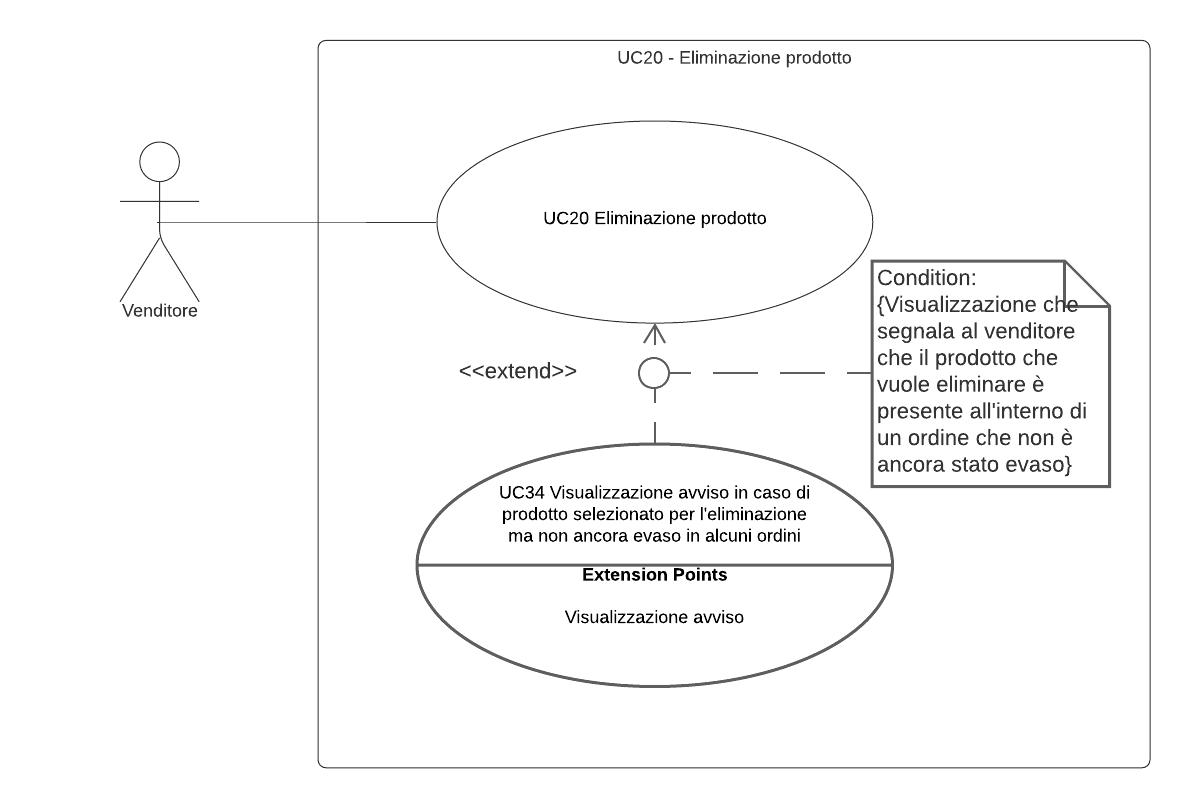
\includegraphics[width=\textwidth]{Immagini/DiagrammiUC/UC20EliminazioneProdotto}
    \caption{Diagramma di \actualUC: Eliminazione di un prodotto da parte del venditore} 
    \label{fig:EliminazioneProdotto}
\end{figure}

Il venditore vuole eliminare un prodotto precedentemente inserito.
\begin{itemize}
    \item \textbf{Attori primari:} venditore;
    \item \textbf{Precondizione:} il venditore si trova nella pagina della dashboard;
    \item \textbf{Postcondizione:} il venditore ha eliminato il prodotto selezionato;
    \item \textbf{Scenario Principale:} il venditore seleziona un prodotto dalla lista di quelli che ha inserito nella piattaforma e preme sul link per eliminarlo definitivamente.
    \begin{itemize}
    \item Il prodotto viene rimosso da PDP, PLP, home, carrelli e dashboard;
    \item Il prodotto rimane negli ordini già effettuati.
    \end{itemize}
    \item \textbf{Estensioni:}
    \begin{enumerate}
    	\item Il venditore seleziona per l'eliminazione, un prodotto che è stato ordinato ma non ancora pagato quindi verrà visualizzato un messaggio di errore e viene negata la possibilità di eliminare il prodotto selezionato.
    \end{enumerate}
\end{itemize}

\UC{Rifornimento prodotto}
Il venditore vuole rifornire un prodotto precedentemente inserito che sta per esaurire o è esaurito.
\begin{itemize}
    \item \textbf{Attori primari:} venditore;
    \item \textbf{Precondizione:} il venditore si trova nella pagina della dashboard;
    \item \textbf{Postcondizione:} il venditore ha rifornito un prodotto;
    \item \textbf{Scenario Principale:} il venditore seleziona un prodotto dalla lista di quelli che ha inserito nella piattaforma e preme sull'azione per rifornirlo. Per completare il rifornimento deve svolgere i seguenti passi:
    \begin{itemize}
        \item (UC) - Inserisce la quantità;
        \item Preme sull'azione per il salvataggio della modifica.
    \end{itemize}
\end{itemize}